\documentclass[11pt]{article}
% --- PREAMBLE ---
% Core packages for typography, math, and layout
\usepackage[utf8]{inputenc}
\usepackage[T1]{fontenc}
\usepackage{lmodern} % Use modern fonts for better rendering
\usepackage[margin=1in]{geometry}
\usepackage{amsmath, amssymb}
\usepackage{graphicx}
\usepackage{booktabs}
\usepackage{caption}
\usepackage[labelfont=bf]{caption}

% Citation and referencing package
\usepackage[numbers, sort&compress]{natbib}

% Hyperlink setup
\usepackage{hyperref}
\hypersetup{
    colorlinks=true,
    linkcolor=blue,
    citecolor=blue,
    filecolor=magenta,
    urlcolor=cyan,
    pdftitle={Eratosthenes’ Experiment: Ancient and Modern Methodology},
    pdfauthor={Daniel Sandner},
}

% Custom math operators for consistency and correct spacing
\DeclareMathOperator{\atan}{arctan}
\DeclareMathOperator{\atanS}{atan2}
\DeclareMathOperator{\hav}{hav}
\DeclareMathOperator{\versin}{versin}

% --- DOCUMENT METADATA ---
\title{\textbf{Eratosthenes’ Experiment: Ancient and Modern Methodology}}
\author{{Daniel Sandner}\thanks{Corresponding author: Daniel Sandner, Independent Researcher, 100 Scientific Visions Initiative, \href{news@sandner.art}{news@sandner.art}}} % Add author information here if available

\date{\today}


\begin{document}

\maketitle

\begin{abstract}
\noindent Eratosthenes' experiment of circa 240 BCE stands as a foundational achievement in geodesy. This paper conducts a rigorous methodological analysis of the experiment, moving beyond its historical outcome to perform a form of scientific archaeology on its methods. We reconstruct the ancient technique, analyzing not only the core geometric insight but also the practical strategies for determining local noon without clocks, and the profound impact of measurement uncertainty. The paper's central historical analysis focuses on the dominant source of error: the distance between Syene and Alexandria. We deconstruct this variable, exploring the ambiguity of the \textit{stadion}, the imprecision of bematist surveys, and a compelling hypothesis of an "informed scientific correction" applied by Eratosthenes himself. This is contrasted with a modern framework detailing enhancements for global application, including corrections for non-aligned points, altitude differences, and sun's declination. Finally, we extend the method's principles into a theoretical tool for comparative planetology, deriving the expected shadow curves for planets of varying geometries. This work reframes Eratosthenes' experiment not as a simple proof, but as a sophisticated and adaptable method for deducing the fundamental properties of a celestial body, both in the ancient world and today.
\end{abstract}

\section{Introduction}

In approximately 240 BCE, Eratosthenes of Cyrene, the chief librarian at the great Library of Alexandria, executed an experiment of remarkable ingenuity and consequence. By observing the difference in solar shadow angles at two locations in Egypt, he produced the first quantitative, evidence-based measurement of the Earth's circumference \cite{Heath1921}. This achievement stands as a foundational moment in the history of science, marking a shift from purely philosophical speculation about the cosmos to its empirical and mathematical measurement. It represents one of the earliest descriptions of successful applications of the scientific method, integrating a theoretical model, precise observation, and geometric calculation to reveal a fundamental truth about the natural world.

The elegance of Eratosthenes' experiment lies in its profound simplicity and its masterful synthesis of existing knowledge with an insightful measurement. The experimental design, known to us primarily through the writings of later authors such as Cleomedes \cite{Cleomedes1990}, was not a complex logistical operation but a brilliant intellectual one. It was predicated on three known facts and one key observation.

First, Eratosthenes, as a master geographer, knew from records and accounts that the city of Syene (modern Aswan) was located on or very near the Tropic of Cancer. This geographical fact meant that at local noon on the day of the summer solstice, the Sun would be directly at the zenith. At this specific moment, vertical objects like an obelisk—or, as Cleomedes anecdotally described, the bottom of a deep well—would be fully illuminated and cast no shadow. This established a \textbf{perfect, zero-angle baseline} for the experiment. Therefore, Eratosthenes did not even need to be in Syene or coordinate with an observer there; he could rely on this well-documented fact.

Second, he knew the approximate overland distance ($d$) between Syene and his own city of Alexandria, which he took to be 5,000 stadia based on the surveys of bematists.

Third, his theoretical model rested on two foundational assumptions: (1) that the Earth is a sphere, and (2) that the Sun is so distant that its rays arrive as basically parallel lines across the globe.

With these three pieces of knowledge, the experiment was reduced to a single, local observation. In Alexandria, at local noon on the same day of the summer solstice, Eratosthenes measured the shadow cast by a gnomon (a vertical rod). He found that the angle of the shadow ($\theta_{\text{Alexandria}}$) was 1/50th of a full circle, or 7.2 degrees.

The geometric insight that followed was the linchpin of the entire discovery (Figure~\ref{fig:geo_rationale}). Because the sun's rays are parallel, the shadow angle measured in Alexandria is, by the principle of alternate interior angles, equal to the central angle ($\Delta\theta$) subtended at the Earth's center by the arc between Syene and Alexandria. The measurement in Alexandria was therefore a direct measurement of the Earth's curvature between the two cities.

The final calculation was straightforward. If the angular separation of $7.2^\circ$ corresponds to a terrestrial distance of 5,000 stadia, then the full $360^\circ$ circumference of the Earth ($C$) would be:
\[
C = \frac{360^\circ}{7.2^\circ} \times 5,000 \text{ stadia} = 50 \times 5,000 \text{ stadia} = 250,000 \text{ stadia}
\]

This result of 250,000 stadia is astonishing, but its true accuracy hinges on the ambiguous length of the \textit{stadion} unit Eratosthenes employed. The modern mean circumference of the Earth is approximately 40,075~km. If Eratosthenes was using the local Egyptian stadion of about 157.5~meters, his measurement translates to \textbf{39,375~km}—an error of less than 2\%. However, if he was using the more common Attic stadion of about 185~meters, his result becomes \textbf{46,250~km}, an overestimate of roughly 15\%. This very uncertainty in the result—ranging from breathtakingly accurate to merely a good estimate—reveals that the most important part of the historical analysis is not the final number, but the reconstruction of the methods, logic, and data Eratosthenes used to obtain it.

\begin{figure}[htbp]
    \centering
    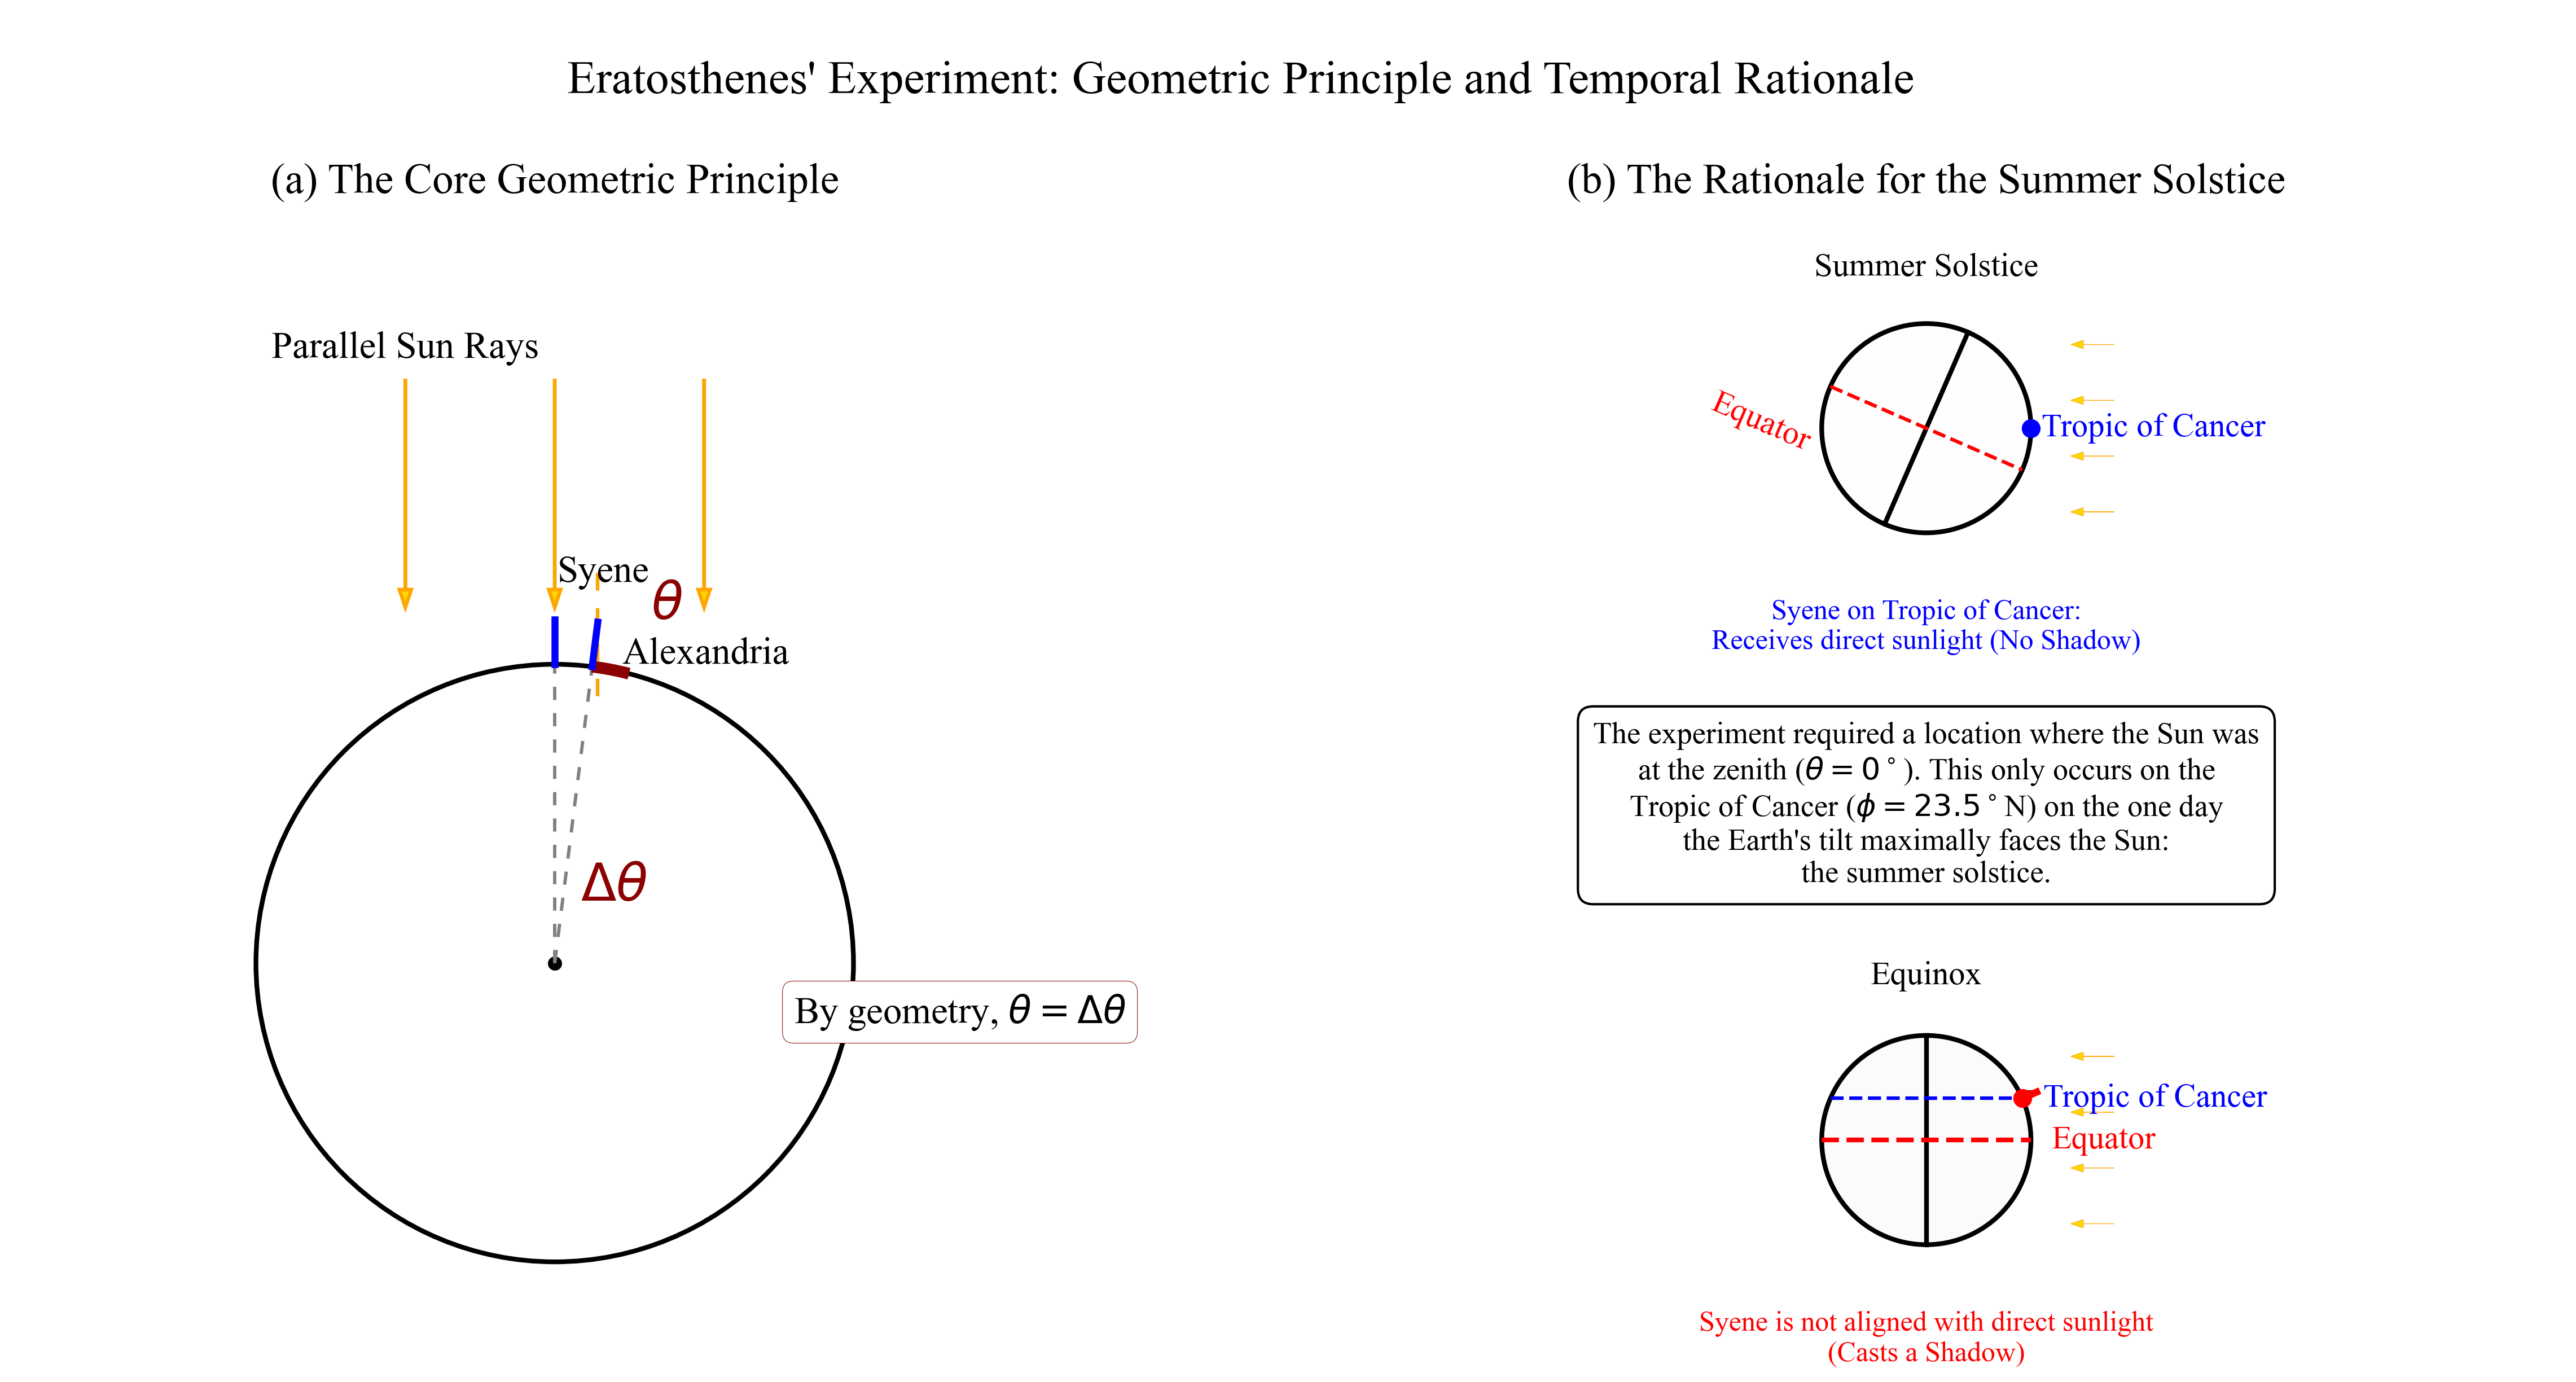
\includegraphics[width=0.9\textwidth]{figures/Eratosthenes_Experiment_Final_Corrected.png}
    \caption{
        The geometric and temporal foundations of Eratosthenes' experiment. 
        \textbf{(a)} The core geometric principle, where the sun's shadow angle at Alexandria ($\theta$) is equal to the central angle between the two cities ($\Delta\theta$) due to the parallel nature of the sun's rays. 
        \textbf{(b)} The temporal rationale, illustrating that only on the summer solstice are the sun's rays perpendicular to the surface at Syene (located on the Tropic of Cancer), creating the necessary zero-shadow condition for the experiment's baseline measurement.
    }
    \label{fig:geo_rationale}
\end{figure}

The purpose of this paper is not simply to recount this famous experiment, but to conduct a deep methodological analysis of it—a form of \textbf{scientific archaeology}. We aim to deconstruct its components to understand not only \textit{how} it worked, but also the practical challenges and sources of uncertainty that defined its execution in the ancient world. The scope of this investigation is threefold: first, to reconstruct the ancient methodology with a focus on the measurement techniques and data-processing strategies Eratosthenes likely employed to manage imperfect information; second, to develop a comprehensive modern framework that refines and generalizes the experiment using contemporary technology and mathematical formalisms; and third, to extend its underlying principles into a theoretical tool for comparative planetology, exploring what this 2,200-year-old method can teach us about discerning the properties of other worlds.

This paper will demonstrate that Eratosthenes' experiment is far from a solved historical curiosity. By dissecting its historical context, sources of error, and theoretical underpinnings, we present a more nuanced portrait of Eratosthenes as a working scientist who grappled with noisy, real-world data. We will move from this reconstruction to outline a high-precision protocol for modern replication, accounting for variables like non-meridian alignment and observer altitude. Finally, we will explore the experiment’s theoretical implications, analyzing the distinct shadow curves produced on planets of differing geometries to show that the method’s true power lies in its adaptability and its ability to reveal the fundamental geometric and astronomical properties of a celestial body.

\section{Historical and Astronomical Foundations}

Eratosthenes' experiment was not an isolated flash of brilliance but the culmination of centuries of intellectual and technical progress across the Hellenistic world and the ancient Near East. His genius lay in his ability to synthesize disparate threads of knowledge—Greek geometric theory, Egyptian observational practice, and Babylonian mathematical astronomy—into a single, elegant experimental design.

\subsection{The Intellectual Milieu of the Library of Alexandria}

As the chief librarian at the Musaeum of Alexandria, Eratosthenes was positioned at the global epicenter of scholarship. The Library was a repository of unprecedented scale, containing maps, astronomical records, mathematical treatises, and travelogues from across the known world. This interdisciplinary environment provided him with the necessary resources: access to the most advanced geometric and astronomical texts, official survey records of the Ptolemaic kingdom, and a culture of critical inquiry that encouraged the application of mathematics to the natural world \cite{MacLeod2004}.

\subsection{Foundational Concepts: The Shoulders of Giants}

A crucial prerequisite for the experiment was a theoretical model of a spherical Earth. This idea, born from philosophy, had been placed on firm observational ground a century before Eratosthenes.

\begin{itemize}
    \item \textbf{Greek Theoretical Framework:} The concept of a spherical Earth is first attributed to Pythagoras (c. 570 BCE) and his school, likely on aesthetic grounds. However, it was Aristotle (384–322 BCE) who provided the first scientific arguments for this model in his treatise \textit{On the Heavens} (\textit{De Caelo}) \cite{Aristotle350BCE}. He cited empirical evidence, including the gradual disappearance of ships' hulls over the horizon, the circular shape of the Earth's shadow on the Moon during a lunar eclipse, and the changing altitude of constellations as one travels north or south. Aristotle concluded, "the Earth is not only round, but it is also a circle of no great size", thus establishing the necessary theoretical basis for a geodetic measurement.

    \item \textbf{Egyptian and Babylonian Technical Legacy:} The practical tools for the experiment were inherited from the older civilizations of the Near East. The gnomon, a simple vertical rod for tracking solar shadows, was a refined version of the monumental obelisks used in Egypt for centuries to mark the solstices and track the sun's daily motion \cite{Pannekoek1961}. From Babylonia came a long tradition of meticulous mathematical astronomy. Babylonian astronomers had developed sophisticated arithmetic methods for predicting celestial events and created extensive observational records, fostering a quantitative and empirical approach to studying the heavens \cite{Neugebauer1957}. However, both cultures operated within a cosmological framework of a flat Earth, which precluded them from using shadow-length variations to measure the planet itself. Eratosthenes' synthesis was in applying these ancient, precise techniques to the new Greek model of a spherical world.
\end{itemize}

\subsection{Primary Historical Accounts}

Eratosthenes' own work on his measurement, likely titled \textit{On the Measurement of the Earth}, has been lost. Our knowledge is therefore reconstructed from later authors who cited his work. These secondary accounts provide the core data for the experiment while also introducing minor variations that reveal the nature of historical and scientific transmission.

\begin{table}[htbp]
\centering
\caption{Key Historical Sources for the Eratosthenes Experiment}
\label{tab:historical_sources}
\small
\begin{tabular}{@{}lp{0.15\linewidth}p{0.5\linewidth}@{}}
\toprule
\textbf{Author (c. Date)} & \textbf{Work} & \textbf{Key Contribution} \\
\midrule
\textbf{Cleomedes} (c. 150 CE) & \textit{On the Circular Motions of the Celestial Bodies} & Provides the most complete description of the method, including the cities of Syene and Alexandria, the observation of a shadowless well, the angle of 1/50\textsuperscript{th} of a circle ($7.2^{\circ}$), and the distance of 5,000 stadia. This is our primary source \cite{Cleomedes150CE}. \\
\addlinespace
\textbf{Strabo} (c. 20 CE) & \textit{Geographica} & A renowned geographer who corroborates the 5,000 stadia distance between the two cities and notes that Syene is located on the Tropic of Cancer \cite{Strabo20CE}. \\
\addlinespace
\textbf{Pliny the Elder} (c. 77 CE) & \textit{Naturalis Historia} & Mentions Eratosthenes' "subtle discovery" and cites a circumference of 252,000 stadia. This slightly different figure may represent a later adjustment by Eratosthenes or others to create a number easily divisible by 60 or 360 \cite{Pliny77CE}. \\
\bottomrule
\end{tabular}
\end{table}

\subsection{Isomorphism and the Cosmological Debate: A Heliocentric Blind Spot}

An important aspect of Eratosthenes’ experiment is its \textbf{isomorphism} with respect to the dominant cosmological models of the day. The experiment's results are identical whether one assumes a geocentric (Earth-centered) or a heliocentric (Sun-centered) system. The underlying geometry depends only on two assumptions: (1) the Earth is spherical, and (2) the Sun is sufficiently far away that its rays arrive as parallel lines. The question of which celestial body is in motion is irrelevant to the measurement of shadow angles at a single instant.

This kinematic equivalence is a primary reason why Eratosthenes' result, while revolutionary, did not challenge the prevailing geocentric model that would later be formalized by Ptolemy. His measurement could be—and was—comfortably absorbed into the geocentric framework by providing the first credible value for the size of the central Earth. This demonstrates a key principle in the history of science: a single experiment, no matter how brilliant, often cannot by itself overturn a well-established paradigm, especially if its results can be incorporated by that paradigm.

It is essential to note that heliocentrism was not an unknown concept. \textbf{Aristarchus of Samos (c. 310 – c. 230 BCE)}, a contemporary of Eratosthenes, had already proposed a fully heliocentric model, arguing that the Earth rotated on its axis and revolved around a stationary Sun. Eratosthenes, working at the center of the Greek intellectual world, was almost certainly aware of Aristarchus's hypothesis \cite{Heath1913}. The fact that his experiment could not distinguish between the two models serves as a perfect illustration of its specific, geodetic focus. It was designed to answer the question "How large is the Earth?", not "What is the Earth's place in the cosmos?".



\section{Reconstruction of the Ancient Methodology: A Study in Uncertainty}

To appreciate the genius of Eratosthenes' experiment, one must reconstruct it not with modern hindsight, but within the constraints of ancient technology and metrology. This requires an analysis of how each component of the experiment was executed and synchronized, and a careful accounting of the sources of uncertainty. We find that the dominant source of error was not in the astronomical observation itself, but in the terrestrial measurement of distance.

\subsection{The Observational Strategy: Synchronizing the Geometric Moment}

A common misconception is that the experiment required a mechanism for precise, simultaneous timekeeping across 800 kilometers. In reality, the experiment required \textbf{geometric synchronization}, not temporal synchronization. The goal was to measure the sun's zenith angle ($\theta$) at both locations at the same geometric instant: the moment the sun crossed the local meridian. This moment, local solar noon, was determined using the gnomon itself.

\subsubsection{Clockless Noon-Finding Techniques}
Ancient observers had two robust methods for identifying local noon without a clock:
\begin{enumerate}
    \item  \textbf{The "Shortest Shadow" Method:} An observer would track the tip of the gnomon's shadow in the hours surrounding midday, marking its path. The point on this curve closest to the gnomon's base marks the shortest shadow, indicating the moment of local noon. The line connecting the gnomon base to this point defines the North-South meridian. While effective, the slow change in shadow length near noon limits its precision to within a few minutes \cite{Goldstein1983}.
    \item  \textbf{The "Method of Equal Altitudes":} A more precise technique involves drawing a circle on a level surface centered at the gnomon's base. The observer marks the two points where the shadow tip crosses this circle, once in the morning and once in the afternoon. The angle bisector of these two points yields a more accurate meridian line, and the temporal midpoint between the two crossings defines local noon with greater precision \cite{Neugebauer1975}.
\end{enumerate}

By using such a method, observers in both Alexandria and Syene could independently ensure their measurements corresponded to the same solar alignment, making absolute time irrelevant.

\subsection{The Critical Variable: Deconstructing the Distance \texorpdfstring{$d$}{d}}

The terrestrial distance ($d$) between Alexandria and Syene is the most significant variable and the largest source of historical uncertainty. Eratosthenes used a value of 5,000 stadia, a figure likely sourced from official records compiled by \textit{bematists}, professional surveyors trained to measure distance by counting their steps. This figure, however, is subject to two distinct layers of uncertainty.

\subsubsection{Layer 1: The Ambiguity of the \textit{Stadion}}
The term "stadion" did not represent a single, universally standardized unit. Its length varied by region and time. Resolving which stadion Eratosthenes used is central to interpreting his result.

\begin{table}[htbp]
\centering
\caption{Common Stadia of the Hellenistic Era}
\label{tab:stadia}
\small
\begin{tabular}{@{}lll@{}}
\toprule
\textbf{Stadion} & \textbf{Length (m)} & \textbf{Context} \\
\midrule
\textbf{Egyptian} & $\sim$157.5 & The local standard in Ptolemaic Egypt, where the experiment was conducted. \\
\addlinespace
\textbf{Olympic} & $\sim$176 & A common standard used in mainland Greece. \\
\addlinespace
\textbf{Attic} & $\sim$185 & The standard used in Athens, widely known in the Greek world. \\
\bottomrule
\end{tabular}
\end{table}

\subsubsection{Layer 2: The Imprecision of the Measurement}
Beyond the unit itself, the number "5,000" is suspiciously round, suggesting it was an official, accepted approximation rather than a precise survey result. The journey, likely following the winding path of the Nile River, was over 900 km long. Even for trained bematists, an error margin of 5--10\% due to terrain and human factors is a reasonable historical assumption \cite{Engels1985}.

\subsection{Reconciling Ancient Data with Modern Measurements}

By comparing the ancient value of 5,000 stadia to modern geodetic data, we can attempt to reverse-engineer Eratosthenes' process and evaluate competing historical hypotheses.

\begin{itemize}
    \item \textbf{Modern Distances:}
    \begin{itemize}
        \item \textbf{Geometric Distance:} The true North-South arc distance between Alexandria ($31.2^{\circ}$N) and Syene ($24.1^{\circ}$N) is approximately \textbf{788 km}. This is the geometrically correct distance for the calculation.
        \item \textbf{Travel Distance:} The path along the Nile is significantly longer, estimated at approximately \textbf{925 km}.
    \end{itemize}
\end{itemize}
\subsubsection{Inferring the Stadion: A Central Conflict}
We can test which stadion Eratosthenes might have used by dividing the known modern distances by his 5,000 stadia figure.
\begin{enumerate}
    \item  If we assume he used the geometrically correct distance:  
    $788,000 \, \text{m} / 5,000 \, \text{stadia} = 157.6 \, \text{m/stadion}$.  
    This provides an almost perfect match for the \textbf{Egyptian stadion}.
    \item  If we assume he used the available travel distance:  
    $925,000 \, \text{m} / 5,000 \, \text{stadia} = 185 \, \text{m/stadion}$.  
    This provides a perfect match for the \textbf{Attic stadion}.
\end{enumerate}

\subsubsection{Three Competing Hypotheses}
This conflict has led to three primary interpretations of Eratosthenes' work:
\begin{enumerate}
    \item \textbf{The "Fortuitous Cancellation of Errors" Hypothesis:} This view suggests Eratosthenes naively used the incorrect travel distance ($\sim$925 km), which was based on the Attic stadion (185 m). The $\sim$17\% overestimate in distance fortuitously compensated for other errors, leading to a surprisingly good result \cite{Dutka1993}.
    \item \textbf{The "Corrupted Data" Hypothesis:} This theory posits that Eratosthenes was a meticulous geodesist. He used the correct Egyptian stadion and a near-correct geometric distance, but his precise angle measurement (closer to the true $7.08^{\circ}$) was rounded to the convenient 1/50\textsuperscript{th} of a circle ($7.2^{\circ}$) by later authors like Cleomedes, who simplified his work \cite{Rawlins1982}.
    \item \textbf{The "Informed Scientific Correction" Hypothesis:} We propose this as the most plausible scenario. Eratosthenes, a master geographer, would have known the bematists' 5,000-stadia travel distance was geometrically flawed. It is highly likely he used his cartographic expertise to apply a scientific correction. Starting with the well-known travel distance (likely in Attic stadia), he could have projected the winding path onto the meridian on his maps, reducing the distance by a reasonable $\sim$10--15\% to arrive at a more accurate geometric value before his final calculation. This portrays him not as lucky or misinterpreted, but as a critical scientist actively refining his imperfect data.
\end{enumerate}


\subsection{An Error Budget for the Ancient Experiment}

To contextualize these issues, a comparative error budget demonstrates that the distance $d$ was the dominant source of uncertainty, dwarfing all other factors.

\begin{table}[htbp]
\centering
\caption{Comparative Error Budget for Eratosthenes' Calculation}
\label{tab:error_budget}
\small
\begin{tabular}{@{}lp{0.3\linewidth}p{0.45\linewidth}@{}}
\toprule
\textbf{Source of Error} & \textbf{Plausible Ancient Uncertainty} & \textbf{Resulting Error in Circumference $C$} \\
\midrule
\textbf{Distance ($d$)} & \textbf{$\sim$10--15\%} (Unit ambiguity \& survey method) & \textbf{$\sim$10--15\%} \\
\addlinespace
\textbf{Angle ($\Delta\theta$)} & \textbf{$\pm0.2^{\circ}$} (Gnomon measurement) & \textbf{$\sim$3--4\%} \\
\addlinespace
\textbf{Meridian Alignment} & Syene is $\sim$$3^{\circ}$ east of Alexandria & \textbf{$<$1\%} (Affects $d$ as non-N-S distance) \\
\addlinespace
\textbf{Altitude Difference} & Negligible in this context & \textbf{$<$0.1\%} \\
\bottomrule
\end{tabular}
\end{table}

This analysis makes it clear that mastering the terrestrial distance was the single greatest challenge of the experiment. The brilliance of Eratosthenes was not only in the experimental design but also in his likely efforts to manage and correct the largest known source of error.

\subsection{Consequences of the Result: Providing a Scale for the Cosmos}

The calculation of the Earth's circumference was not an intellectual exercise in isolation; it had profound, cascading effects on the quantitative science of astronomy. By providing a reliable value for the Earth's radius ($R$), Eratosthenes provided the first rung on the "cosmic distance ladder." His result was the fundamental baseline—the "meter stick"—that allowed astronomers to convert relative distances into absolute ones.
\begin{enumerate}
    \item  \textbf{Calculating the Distance to the Moon:} Aristarchus had previously devised a geometric method to estimate the Moon's distance in terms of Earth radii. By observing the size and curvature of the Earth's shadow on the Moon during a lunar eclipse, he estimated the Moon’s distance to be approximately 60 Earth radii \cite{Dreyer1953}. This was a brilliant, but purely relative, result. Once Eratosthenes calculated $C \approx 252,000$ stadia, a value for $R$ became known ($R = C / 2\pi$). Astronomers could, for the first time, assign a plausible absolute distance to a celestial body:
    \[
    \text{Distance to Moon} \approx 60 \times \frac{252,000}{2\pi} \, \text{stadia} \approx 2,400,000 \, \text{stadia.}
    \]
    This was the first scientifically-grounded estimate of the size of the Earth-Moon system.

    \item  \textbf{Estimating the Distance to the Sun:} Aristarchus had also attempted to find the Sun's distance relative to the Moon's. By measuring the angle between the Sun and a half-moon (when the Earth-Moon-Sun angle is $90^{\circ}$), he estimated the Sun was about 19 times farther away than the Moon. While his measurement was imprecise (the true ratio is closer to 400), it established that the Sun was much farther and therefore vastly larger than the Earth. Eratosthenes' result allowed this ratio to be converted into an absolute, albeit underestimated, distance. This provided the first quantitative evidence that the Earth was not the dominant body in the solar system, a key piece of evidence for the (unpopular) heliocentric model.

    \item  \textbf{Foundation for Mathematical Geography:} A known circumference is the prerequisite for a global system of latitude and longitude. Eratosthenes himself pioneered this, creating world maps that featured, for the first time, a grid of perpendicular lines based on a spherical Earth of known size. This transformed cartography from a descriptive art into a mathematical science \cite{Berggren2000}.
\end{enumerate}

In summary, Eratosthenes' measurement was the critical linchpin that connected terrestrial geometry with cosmic geometry. It grounded astronomical models in a physical, measurable reality and enabled the first quantitative, scaled estimates of the cosmos.

\section{Modern Methodological Enhancements}

While Eratosthenes’ method was revolutionary, its reliance on specific simplifying assumptions (meridian alignment, solstice date) limited its general applicability. A modern reconstruction of the experiment can remove these constraints through the application of precise instrumentation and spherical trigonometry, transforming it into a robust and globally applicable geodetic tool. This section outlines a high-precision protocol for a modern experiment and quantifies the corrections for factors negligible in antiquity but relevant today.

\subsection{A Generalized Framework for Global Measurement}

The core of the modern method is to generalize the experiment for any two points on Earth ($P_1$ and $P_2$), measured on any given day. This requires a departure from local noon and an introduction of universal time.

\subsubsection{Independence from Meridian Alignment}
Eratosthenes chose two cities he believed to be on the same meridian to simplify the distance $d$ into a pure North-South arc. For two arbitrarily located points, $P_1(\phi_1, \lambda_1)$ and $P_2(\phi_2, \lambda_2)$, where $\phi$ is latitude and $\lambda$ is longitude, the relevant distance is the great-circle path. This distance, $d$, can be calculated with high precision using the \textbf{haversine formula} \cite{Sinnott1984}:
\begin{gather}
    a = \sin^2(\Delta\phi/2) + \cos(\phi_1)\cos(\phi_2)\sin^2(\Delta\lambda/2) \label{eq:haversine_a} \\
    c = 2 \cdot \atanS(\sqrt{a}, \sqrt{1-a}) \label{eq:haversine_c} \\
    d = R \cdot c 
    \label{eq:haversine_d}
\end{gather}
Where $\Delta\phi = \phi_2 - \phi_1$, $\Delta\lambda = \lambda_2 - \lambda_1$, and $R$ is the Earth's mean radius ($\sim$6,371 km). All angles must be in radians.

\subsubsection{Independence from the Solstice: Accounting for Solar Declination}
To conduct the experiment on any day, one must account for the sun’s declination, $\delta$, which is the angle of the sun's rays relative to the Earth's equatorial plane. The zenith angle $\theta$ at a specific location is no longer equal to its latitude, but is given by \cite{Meeus1998}:
\begin{equation}
    \theta = |\phi - \delta|
    \label{eq:zenith_declination}
\end{equation}
The declination $\delta$ for any given day of the year ($N$) can be approximated by the formula:
\begin{equation}
    \delta \approx -23.45^{\circ} \times \cos\left( \frac{360^{\circ}}{365} \cdot (N + 10) \right)
    \label{eq:declination}
\end{equation}
or obtained from astronomical almanacs for higher precision.

\subsubsection{Synchronized Measurement}
Since the two points are not on the same meridian, their local noons differ. It is therefore essential that the measurement of the sun's shadow be taken at both locations at the \textbf{same instant of universal time} (e.g., 12:00 UTC). This ensures that the measured shadow angles correspond to a single, fixed position of the sun relative to the Earth, making the subsequent geometric calculation valid.

\subsection{A High-Precision Protocol}

A modern experiment would follow these steps:
\begin{enumerate}
    \item \textbf{Site Selection:} Choose two or more locations with precisely known coordinates ($\phi$, $\lambda$) and altitudes ($h$).
    \item \textbf{Instrumentation:} Use a theodolite or a smartphone application with a digital inclinometer to measure the sun's altitude ($\alpha$) directly, or use a precision-machined gnomon on a leveled surface to measure shadow length ($s$).
    \item \textbf{Data Acquisition:} At a pre-agreed universal time, all observers measure the sun's altitude $\alpha$ or shadow length $s$. The zenith angle is then calculated as $\theta = 90^{\circ} - \alpha$ or $\theta = \atan(s/h)$.
    \item \textbf{Calculation:}
    \begin{enumerate}
        \item Determine the angular separation of the sun's rays as they strike the Earth, $\Delta\theta$, which is the great-circle angle between the two sub-solar points. In a simplified but effective approach, $\Delta\theta$ can be approximated by the angle between the two measured zenith vectors.
        \item Calculate the great-circle distance $d$ between the two observation points using their coordinates and the haversine formula (Eq. \ref{eq:haversine_d}).
        \item Calculate the circumference using the foundational formula: $C = (360^{\circ}/\Delta\theta) \cdot d$.
    \end{enumerate}
    \item \textbf{Data Aggregation:} If using a network of three or more points, calculate the circumference for multiple pairs and average the results to reduce random measurement error.
\end{enumerate}

\subsection{Correction for Second-Order Effects}
For a truly rigorous measurement aiming for the highest accuracy, two further corrections are necessary.

\subsubsection{Observer Altitude}
Observers are not at sea level. They measure a distance $d_{\text{ground}}$ on a circle of radius $R + h$, where $h$ is their average altitude. To find the Earth's sea-level circumference, this distance must be mathematically reduced. The corrected sea-level distance, $d_{\text{sea}}$, is given by \cite{Vanicek1986}:
\begin{equation}
    d_{\text{sea}} \approx d_{\text{ground}} \cdot \left(\frac{R_{\text{sea}}}{R_{\text{sea}} + h_{\text{avg}}}\right)
    \label{eq:altitude_correction}
\end{equation}
While this correction is small ($\sim$0.025\% for an altitude of 1.6 km), it is essential for precision geodesy.

\subsubsection{Earth's Oblateness}
The Earth is not a perfect sphere but an oblate spheroid, with an equatorial radius ($\sim$6,378 km) that is $\sim$21 km larger than its polar radius ($\sim$6,357 km). This has two effects:
\begin{enumerate}
    \item The Earth's radius $R$ is latitude-dependent.
    \item The local vertical (defined by a plumb line) does not point directly to the Earth's geometric center, except at the equator and the poles. The difference is the \textit{deflection of the vertical}.
\end{enumerate}
A full geodetic treatment would use a more complex model like the WGS84 reference ellipsoid instead of a simple sphere. However, for most applications outside of professional geodesy, using the mean radius in the haversine formula provides a result well within 1\% of the true value, which is sufficient for demonstrating the method's power and precision \cite{Torge2012}.

\begin{table}[htbp]
\centering
\caption{Comparison of Ancient vs. Modern Methodological Components}
\label{tab:ancient_vs_modern}
\small
\begin{tabular}{@{}lp{0.25\linewidth}p{0.25\linewidth}p{0.35\linewidth}@{}}
\toprule
\textbf{Component} & \textbf{Ancient Method} & \textbf{Modern Method} & \textbf{Rationale for Enhancement} \\
\midrule
\textbf{Synchronization} & Local Noon (Geometric) & Universal Time (UTC) & Enables measurement between non-aligned points. \\
\addlinespace
\textbf{Distance ($d$)} & Bematist survey, estimated & GPS and Haversine Formula & Eliminates the largest source of error and uncertainty. \\
\addlinespace
\textbf{Angle ($\Delta\theta$)} & Gnomon, solstice observation & Theodolite/App, declination formula & Allows measurement on any day and increases precision. \\
\addlinespace
\textbf{Altitude ($h$)} & Ignored (negligible effect) & Mathematically corrected & Required for high-precision geodetic results. \\
\addlinespace
\textbf{Earth Model} & Perfect Sphere & Oblate Spheroid (e.g., WGS84) & Increases accuracy by using a more realistic model of Earth's shape. \\
\bottomrule
\end{tabular}
\end{table}

\section{Theoretical Analysis: The Experiment on Other Worlds}

The true power of Eratosthenes’ method lies not in its historical result, but in its universal principles. By abstracting the experiment from its terrestrial context, we can reframe it as a fundamental geodetic tool applicable to any planet illuminated by a star. The relationship between a planet's geometry, its star's position, and the resulting shadow lengths forms a unique signature. This section explores these signatures, deriving the theoretical shadow curves for planets of different shapes and considering the impact of varying solar system configurations.

\subsection{Shadow Curves as Geometric Signatures}

The core insight is that a simple, measurable quantity—the length of a gnomon's shadow—is a direct function of the planet’s global curvature. By measuring how shadow length varies with distance from a subsolar point, an observer can deduce the underlying geometry of their world. For this analysis, we assume a gnomon of height $h = 1$ unit, an equinox condition where the star is directly over the equator (declination $\delta = 0^{\circ}$), and observers at local noon.

\subsubsection{Spherical Planet (Baseline)}
On a spherical planet, the zenith angle $\theta$ of the star is equal to the observer's latitude $\phi$. The relationship between the gnomon $h$, its shadow $s$, and the zenith angle $\theta$ forms a right triangle. The shadow length is therefore given by the tangent function \cite{Cox2011}:
\begin{equation}
    s(\phi) = h \cdot \tan(\phi) = \tan(\phi)
    \label{eq:shadow_sphere}
\end{equation}
The curve is non-linear, growing moderately at low latitudes and accelerating towards infinity as the latitude approaches $90^{\circ}$. This trigonometric relationship is a direct consequence of Euclidean geometry on a curved surface.

\subsubsection{Flat Planet}
On a flat-plane world, the sun is not infinitely distant but located at a finite altitude $H$. The shadow length $s$ depends on the observer's linear distance $d$ from the subsolar point. By similar triangles:
\begin{equation}
    s/h = d/H \quad \implies \quad s(d) = d/H
    \label{eq:shadow_flat}
\end{equation}
The shadow curve is perfectly linear. To compare this to the spherical case, we can approximate the linear distance $d$ from the "latitude" $\phi$, assuming a planet with an Earth-like circumference ($C \approx 40,000$ km). Then $d = (\phi/360) \cdot C$. Assuming a typical flat-Earth sun altitude of $H = 5,000$ km, the shadow length is:
\[
s(\phi) = \frac{ (\phi \cdot 40000) / 360 }{5000} = \frac{\phi \cdot 8}{360} = \frac{\phi}{45}
\]

\subsubsection{Replicating Spherical Results on a Flat World: The Physical Requirements}
For a flat-Earth model to yield the same shadow measurements as a spherical one, it cannot rely on consistent physical laws. The linear nature of its shadow curve ($s = d/H$) must be forced to mimic the non-linear, trigonometric curve of the spherical model ($s = \tan(\phi)$). This requires introducing ad-hoc physical conditions that are not globally consistent. The primary way to achieve this is to abandon the assumption of a constant solar altitude ($H$) and allow it to vary as a function of the observer's location. By setting the two shadow equations equal, we can derive the required altitude $H$ for any given location $\phi$:
\begin{equation}
    \tan(\phi) = d/H \quad \implies \quad H(\phi) = d / \tan(\phi)
    \label{eq:H_phi}
\end{equation}
Where $d$ is the linear distance from the subsolar point, itself a function of latitude ($d \approx (\phi/360) \cdot C$). This leads to a physically implausible requirement: the sun's altitude would have to systematically \textbf{decrease} as an observer moves away from the equator to higher latitudes. This ad-hoc model would not be consistent across the entire flat surface. A single, physical sun cannot have multiple altitudes simultaneously. The model can be tuned to provide a \textit{local fit} for any two points, but it fails as a \textit{global model}. This internal inconsistency demonstrates that the flat-Earth model must be rejected on the grounds of falsifiability when multiple data points are introduced \cite{Popper1959}.

\subsubsection{The Ambiguity of a Two-Point Measurement and the Power of a Third}
For the sake of scientific accuracy, it must be noted that an Eratosthenes experiment performed between \textbf{only two points does not, by itself, definitively prove a spherical shape}. With only two data points, both models are internally valid explanations. The power to falsify one of these models emerges with the introduction of a \textbf{third measurement point}.
\begin{itemize}
    \item In the \textbf{spherical model}, the third measurement will fall along the same $\tan(\phi)$ curve predicted by the first two points. Pairwise calculations between points (1,3) and (2,3) will yield the same circumference $C$ as the (1,2) calculation, demonstrating global consistency.
    \item In the \textbf{flat model}, the third measurement will \textbf{not} lie on the linear $d/H$ curve defined by the first two points. Calculating the solar altitude $H$ using a new pair of points will yield a different value, proving the model is inconsistent and therefore incorrect.
\end{itemize}
Therefore, while a two-point experiment can \textit{measure} a property (like circumference or solar altitude) \textit{within a given model}, it is a \textbf{multi-point experiment ($n \ge 3$) that can scientifically distinguish between competing models of planetary geometry}.

\subsubsection{Hypothetical Geometries}
\begin{enumerate}
    \item  \textbf{Hyperbolic Planet:} A hyperbolic geometry is characterized by negative curvature (a "saddle" shape). On such a surface, parallel lines diverge. The effect on shadow lengths would be an even more extreme divergence than on a sphere. The trigonometric relationship would be replaced by a hyperbolic function, likely causing the shadow length to grow super-linearly, even faster than $\tan(\phi)$ \cite{Richards1997}.
    \item  \textbf{Inverted Spheroid (Concave World):} In this speculative model, observers live on the inner surface of a sphere. Light propagation becomes complex, but assuming straight-line rays from a central sun, observers at higher "latitudes" would be angled \textit{towards} the sun's rays. This would cause shadows to behave erratically, potentially shortening at higher latitudes, a direct contradiction to all real-world observation.
\end{enumerate}

\begin{table}[htbp]
\centering
\caption{Comparative Shadow Lengths ($s$) for Different Planetary Models ($h=1$)}
\label{tab:model_comparison}
\small
\begin{tabular}{@{}cccc@{}}
\toprule
\textbf{"Latitude" $\phi$} & \textbf{Spherical $s = \tan(\phi)$} & \textbf{Flat $s = \phi/45$ ($H=5000$km)} & \textbf{Qualitative Hyperbolic Behavior} \\
\midrule
\textbf{$0^{\circ}$} & 0.00 & 0.00 & $\sim$0 \\
\textbf{$30^{\circ}$} & 0.58 & 0.67 & Similar to spherical \\
\textbf{$60^{\circ}$} & 1.73 & 1.33 & Noticeably longer than spherical \\
\textbf{$80^{\circ}$} & 5.67 & 1.78 & Dramatically longer \\
\textbf{$89^{\circ}$} & 57.29 & 1.98 & Approaching infinity much faster \\
\bottomrule
\end{tabular}
\end{table}

This comparison demonstrates that a simple multi-point Eratosthenes-style experiment, plotting shadow length against distance, can definitively distinguish between competing models of planetary geometry without ambiguity.

\subsection{Impact of Solar System Configuration}

\subsubsection{Close Primary Star: Breakdown of the Parallel-Ray Assumption}
The assumption that the star's rays are parallel is an excellent approximation for the Earth-Sun system, where the sun's distance ($\sim$150 million km) is over 10,000 times the Earth's diameter. If a planet were orbiting much closer to its star, this assumption would fail. The incoming rays would have a noticeable divergence, a phenomenon known as \textbf{solar parallax} \cite{Anderson1999}. The experiment, in this case, could be modified to solve for two unknowns simultaneously: the planet's radius $R$ and its distance from its star $D$.

\subsubsection{Binary Star Systems}
An experiment on a planet illuminated by two stars would present a unique observational challenge: the presence of two overlapping shadows (\textit{penumbrae}) for any given object. The method could be adapted:
\begin{enumerate}
    \item \textbf{Filtering:} If the two stars have different spectral types, an observer could use an optical filter to block the light from one star, allowing the shadow cast by the other to be measured cleanly.
    \item \textbf{Timing:} If the planet is in a non-synchronous orbit, there may be times when one star is eclipsed by the other, or when one has set while the other is still in the sky, providing a window for an unambiguous measurement.
\end{enumerate}
This theoretical analysis shows that the Eratosthenes experiment is not merely a historical anecdote but a foundational principle of planetary science.

\section{Conclusion}

Eratosthenes' measurement of the Earth's circumference was more than a brilliant calculation; it was a testament to the power of the scientific method. This paper has conducted a deep methodological analysis of this landmark experiment, moving beyond the historical result to dissect its scientific process.

Our reconstruction of the ancient methodology revealed that the experiment's success hinged on a sophisticated understanding of measurement and uncertainty. We have shown that Eratosthenes did not require absolute timekeeping, but rather a precise geometric synchronization. The primary source of uncertainty was not in the astronomical angle, but in the terrestrial distance. Our analysis led to the "Informed Scientific Correction" hypothesis, portraying Eratosthenes not as a lucky theorist, but as a critical scientist who likely understood the limitations of his raw data and applied a reasoned, cartographic correction.

Contrasting this ancient practice with a modern framework highlighted the experiment's adaptability. By incorporating universal time, spherical trigonometry, and corrections for factors like solar declination and observer altitude, the method is transformed into a precise and globally applicable geodetic tool. Finally, our theoretical analysis reframed the experiment as a universal instrument for comparative planetology. We have demonstrated that the shadow curves produced on planets of different geometries—spherical, flat, or hyperbolic—are unique and distinguishable.

Ultimately, this investigation reaffirms the enduring relevance of Eratosthenes' work. It is not an obsolete historical anecdote, but a living scientific principle. It serves as a powerful educational tool, a case study in scientific reasoning and error analysis, and a foundational concept for understanding how we measure and map any world. The experiment's true legacy is its elegant demonstration that with a simple stick, a shadow, and a mastery of reason, it is possible to measure the world.

% --- BIBLIOGRAPHY ---
\bibliographystyle{plainnat}
\bibliography{references}


% --- APPENDICES ---
\appendix
\section{Mathematical Derivations}

The main body of this paper relies on several key mathematical formulae. This appendix provides the formal derivations for these essential equations, serving as a self-contained reference for the geometric and trigonometric principles at play.

\subsection{The Haversine Formula for Great-Circle Distance}

The haversine formula is a numerically stable method for calculating the great-circle distance between two points on a sphere, avoiding issues with small angles that can arise with the spherical law of cosines.

\begin{itemize}
    \item \textbf{Definitions:}
    \begin{itemize}
        \item The \textbf{versine} (versed sine) of an angle $\theta$ is $\versin(\theta) = 1 - \cos(\theta)$.
        \item The \textbf{haversine} (half-versine) is $\hav(\theta) = \versin(\theta) / 2 = (1 - \cos(\theta)) / 2 = \sin^2(\theta/2)$.
        \item Let two points be $P_1(\phi_1, \lambda_1)$ and $P_2(\phi_2, \lambda_2)$, where $\phi$ is latitude and $\lambda$ is longitude.
        \item Let $c$ be the angular distance between the two points, and $R$ be the sphere's radius.
    \end{itemize}
    \item \textbf{Derivation:}
    Consider the spherical triangle formed by the North Pole ($N$) and the two points $P_1$ and $P_2$. The sides of this triangle are the angular distances: $a = (\pi/2) - \phi_2$ and $b = (\pi/2) - \phi_1$. The angle at the North Pole, $N$, is the difference in longitudes, $\Delta\lambda = \lambda_2 - \lambda_1$. Applying the \textbf{spherical law of cosines}:
    \[
    \cos(c) = \cos(a)\cos(b) + \sin(a)\sin(b)\cos(N)
    \]
    Substituting the co-latitudes:
    \[
    \cos(c) = \sin(\phi_2)\sin(\phi_1) + \cos(\phi_2)\cos(\phi_1)\cos(\Delta\lambda)
    \]
    To derive the haversine formula, start with $\hav(c) = (1 - \cos(c)) / 2$:
    \[
    \hav(c) = \frac{1 - (\sin(\phi_1)\sin(\phi_2) + \cos(\phi_1)\cos(\phi_2)\cos(\Delta\lambda))}{2}
    \]
    Using the identity $\cos(\Delta\lambda) = 1 - 2\hav(\Delta\lambda)$ and $1 - \cos(\phi_1 - \phi_2) = 2\hav(\phi_1 - \phi_2)$:
    \[
    \hav(c) = \hav(\phi_1 - \phi_2) + \cos(\phi_1)\cos(\phi_2)\hav(\Delta\lambda)
    \]
    Recalling that $\hav(\theta) = \sin^2(\theta/2)$, we arrive at the final form:
    \[
    \sin^2(c/2) = \sin^2(\Delta\phi/2) + \cos(\phi_1)\cos(\phi_2)\sin^2(\Delta\lambda/2)
    \]
    The great-circle distance is $d = R \cdot c$.
\end{itemize}

\subsection{Formula for Solar Declination}
The solar declination $\delta$ is the angle between the sun's rays and the plane of the Earth's equator. It is a function of the Earth's axial tilt ($\epsilon \approx 23.45^{\circ}$) and its orbital position.
\begin{itemize}
    \item \textbf{Definitions:} $\epsilon$: Earth's axial tilt ($\approx 23.45^{\circ}$); $N$: The day of the year.
    \item \textbf{Derivation:} The declination can be modeled as a cosine function. The term $(N+10)$ provides a phase shift to align the curve with the calendar, placing the Northern Hemisphere's winter solstice (where $\delta \approx -\epsilon$) around day 355.
    \[
    \delta(N) \approx -\epsilon \cdot \cos\left( \frac{360^{\circ}}{365.25} \cdot (N + 10) \right)
    \]
    For example, at the vernal equinox ($N \approx 81$), the argument of cosine is $\approx 90^{\circ}$, yielding $\delta \approx 0^{\circ}$. At the summer solstice ($N \approx 172$), the argument is $\approx 180^{\circ}$, yielding $\delta \approx +\epsilon$.
\end{itemize}

\subsection{Derivation of the Altitude Correction for Arc Distance}
This reduces a measured ground distance to its sea-level equivalent.
\begin{itemize}
    \item \textbf{Definitions:} $R_{\text{sea}}$ is sea-level radius; $h_{\text{avg}}$ is average altitude; $d_{\text{ground}}$ is measured arc distance; $d_{\text{sea}}$ is sea-level distance; $c$ is the central angle.
    \item \textbf{Derivation:} Arc length is $d = R \cdot c$. For the measurement at altitude: $d_{\text{ground}} = (R_{\text{sea}} + h_{\text{avg}}) \cdot c$. For the equivalent distance at sea level: $d_{\text{sea}} = R_{\text{sea}} \cdot c$. We express $c$ from the first equation, $c = d_{\text{ground}} / (R_{\text{sea}} + h_{\text{avg}})$, and substitute into the second:
    \[
    d_{\text{sea}} = d_{\text{ground}} \cdot \left( \frac{R_{\text{sea}}}{R_{\text{sea}} + h_{\text{avg}}} \right)
    \]
\end{itemize}

\subsection{Derivation of Zenith Angle from Gnomon Measurements}
\begin{itemize}
    \item \textbf{Definitions:} $h$ is the vertical gnomon height; $s$ is the horizontal shadow length; $\theta$ is the sun's zenith angle.
    \item \textbf{Derivation:} The gnomon, shadow, and sun's ray form a right-angled triangle. By definition of the tangent function:
    \[
    \tan(\theta) = \frac{\text{opposite}}{\text{adjacent}} = \frac{s}{h} \implies \theta = \atan\left(\frac{s}{h}\right)
    \]
\end{itemize}

\subsection{Derivation of Solar Altitude for Flat-Earth Model}
This calculates the required solar altitude $H$ between any two points on a flat plane.
\begin{itemize}
    \item \textbf{Definitions:} $d$ is linear distance between points $P_1, P_2$; $s_1, s_2$ are shadow lengths; $h$ is gnomon height; $H$ is solar altitude; $d_1, d_2$ are distances from the subsolar point.
    \item \textbf{Derivation:} From similar triangles: $s_1 / h = d_1 / H \implies d_1 = H \cdot (s_1 / h)$, and similarly for point 2. Assuming collinear points, $d = |d_1 - d_2|$.
    \[
    d = \left| H \cdot \frac{s_1}{h} - H \cdot \frac{s_2}{h} \right| = \frac{H}{h} |s_1 - s_2|
    \]
    Solving for $H$:
    \[
    H = \frac{d \cdot h}{|s_1 - s_2|}
    \]
    The flat-Earth hypothesis is falsified if $H$ is not constant for different pairs of points.
\end{itemize}

\subsubsection*{Conclusion to Appendix A}
The derivations presented in this appendix collectively form the mathematical backbone of the paper's analysis. Together, these mathematical formalisms ensure that the paper's conclusions are not merely descriptive but are grounded in robust, verifiable geometric and astronomical principles.

\section*{Appendix B: Comparative Metrological Data}

This appendix provides quantitative data to support the analysis of Eratosthenes' experiment and the physical realities of Earth's geometry. Its primary purpose is to illustrate how the planet's curvature, which is negligible at human scales, becomes a decisive factor over the geodetic distances involved in the ancient measurement.

\subsection*{The Formula for Curvature Drop}

To quantify the effect of curvature, we can calculate the "curvature drop" ($h_{\text{drop}}$). This is the vertical distance a point on the Earth's surface "drops" away from a perfectly straight, tangential line extending from an observer's position. For a given geodetic (great-circle) distance $d$ and a planetary radius $R$, this drop can be accurately approximated by the formula:
\[
h_{\text{drop}} \approx \frac{d^2}{2R}
\]
This approximation is derived from the Pythagorean theorem and is highly accurate for distances up to several thousand kilometers. For all calculations in Table B.2, we use the Earth's mean radius, $R \approx 6,371$ km.

\subsection*{Tables of Conversion and Curvature}

To contextualize the calculations, Table~B.1 provides the key conversion factors for the Hellenistic stadia discussed in this paper. Table~B.2 then applies these conversions and the curvature formula to a range of distances, from a short 10 km to well beyond the scale of Eratosthenes' experiment, showing how the deviation from a flat plane grows quadratically with distance.

\begin{table}[htbp]
\centering
\caption{Hellenistic Stadia and Modern Equivalents}
\label{tab:stadia_conversion}
\small
\begin{tabular}{@{}lccc@{}}
\toprule
\textbf{Stadion Name} & \textbf{Length (m)} & \textbf{km per Stadion} & \textbf{Miles per Stadion} \\
\midrule
\textbf{Egyptian} & $\approx 157.5$ & 0.1575 & $\approx 0.0979$ \\
\textbf{Attic}    & $\approx 185.0$ & 0.1850 & $\approx 0.1150$ \\
\bottomrule
\end{tabular}
\end{table}

\begin{table}[htbp]
\centering
\caption{Earth's Curvature Drop over Geodetic Distances}
\label{tab:curvature_drop}
\small
\begin{tabular}{@{}rrrrrr@{}}
\toprule
\multicolumn{2}{c}{\textbf{Distance (Stadia)}} & \multicolumn{2}{c}{\textbf{Geodetic Distance}} & \multicolumn{2}{c}{\textbf{Curvature Drop ($h_{\text{drop}}$)}} \\
\cmidrule(r){1-2} \cmidrule(lr){3-4} \cmidrule(l){5-6}
\textbf{Egyptian} & \textbf{Attic} & \textbf{Kilometers} & \textbf{Miles} & \textbf{Meters} & \textbf{Feet} \\
\midrule
64 & 54 & 10 & 6.2 & $\approx 7.8$ & $\approx 26$ \\
635 & 541 & 100 & 62.1 & $\approx 785$ & $\approx 2,575$ \\
\addlinespace
\textbf{5,000} & 4,257 & \textbf{787.5} & 489.3 & $\approx 48,680$ & $\approx 159,711$ \\
5,937 & \textbf{5,000} & \textbf{925.0} & 574.8 & $\approx 67,000$ & $\approx 219,816$ \\
\addlinespace
12,700 & 10,000 & 1,850 & 1,150 & $\approx 268,000$ & $\approx 879,265$ \\
25,400 & 20,000 & 3,700 & 2,300 & $\approx 1,072,000$ & $\approx 3,517,060$ \\
\bottomrule
\end{tabular}
\captionsetup{font=small, justification=justified}
\caption*{
\textbf{Notes:} This table demonstrates the dramatic, non-linear increase in curvature drop with distance. At 10 km, the drop is less than 8 meters. At the 788 km distance of the experiment, the drop is over 48 kilometers (nearly 30 miles), a monumental deviation from a flat plane that is easily measurable. The key experimental distances are highlighted in bold. Curvature is calculated using $h_{\text{drop}} \approx d^2/(2R)$ with $R = 6371$ km.
}
\end{table}

\subsubsection*{Conclusion to Appendix B}

The data presented here numerically substantiates the foundational premise of Eratosthenes' work. While the Earth appears flat over short, everyday distances, its spherical nature produces a significant and measurable geometric effect over the hundreds of kilometers separating cities. Table~B.2 makes it clear that any model of the world used for long-distance cartography or geodesy must account for this curvature to have any correspondence with reality. 

\end{document}